\documentclass[twocolumn]{article}
\usepackage{pgfplots}
\usepgfplotslibrary{groupplots}
\pgfplotsset{compat=1.16}
\usepackage{color}
\usepackage[top=1in,bottom=1in,left=1.2in,right=1.2in]{geometry}
\usepackage{hyperref}
\usepackage{natbib}
\usepackage[small]{titlesec}
\usepackage{nicematrix}
\usepackage{graphicx}
\usepackage{rotating}
\usepackage[dvipsnames]{xcolor}
\usepackage{amsmath}
\usepackage[]{minted}
\usepackage{float}
\newenvironment{code}{\captionsetup{type=listing}}

\newcommand{\tcode}[1]{\texttt{#1}}

\setminted{breaklines=true, fontsize=\small}

\title{Comparative Analysis of Prompting Techniques for Text Classification Across Multiple LLMs \\ \begin{small}\url{https://github.com/jaydent22/661-final-project}\end{small}}
\author{Ethan Chung, Jayden Tactay, Samuel Yang}

\date{}

\begin{document}
\maketitle

\section{Introduction}

Due to the complexity of natural language, with correct categorization relying on understanding the nuanced context of a word or sentence, text classification is a challenging task for language models with no inherent understanding of language. This challenge is apparent, and even amplified, when attempting to effectively prompt these models for some specific task.

Especially with techniques like zero-shot, few-shot, and chain-of-thought (CoT) prompting, it becomes imperative to both choose an appropriate technique for the task and design an effective prompt for optimal performance; yet, how can we determine which technique is "appropriate" for our task, and how do we design an "effective" prompt? What determines an "effective" prompt? We aim to gain insight into these questions by comparing prompting techniques on various text classification datasets with different large language models, and investigating the difference in performance between different prompting techniques on different models and datasets.

We test CoT, few-shot, and zero-shot prompting on the following models: LLAMA 3.1, GPT-Neo, and Yi 1.5. LLAMA 3.1 is the most recent versions of Meta’s LLAMA model family; compared to an older model like GPT-Neo or a model with a different targeted use case like 01-ai’s Yi 1.5 models (i.e., bilingual English and Chinese language modeling), we expect different prompting strategies to yield different results.

We use the following datasets in our experiments: Stanford Sentiment Treebank v2 (SST-2), Contextualized Affect Representations for Emotion Recognition (CARER), and the Hate Speech Dataset from a White Supremacy Forum.

Using iterative prompt design and modification, we prompt the models to perform classification on each dataset and determine the effectiveness of the various prompting strategies/changes. To provide benchmarks with which to compare model performance, we fine-tune T5 and BART models and obtain a human performance metric on each dataset. To provide a more consistent performance comparison, we prompt the language models on the same test datasets used to assess the baseline models, using examples from the training datasets for few-shot and CoT prompts. In this study, we reinforce that model performance is dependent on both prompt design and model training bias. We also highlight that large language models are contextual reasoners, performing worse in the absence of relevant context.

\section{Data}

The SST-2 dataset, introduced by Socher et. al (2013), is the binarized version of a corpus of parse trees for sentiment analysis on sentence parts. The dataset consists of various sentence constituents of movie reviews, each given a label of either positive or negative. The dataset available on Hugging Face consists of 67349 training examples, 872 validation examples, and 1821 test examples. The training split is mostly balanced, with both labels having a nearly 50\% representation. As the SST-2 dataset is used as a General Language Understanding Evaluation (GLUE) benchmark task, the test labels are hidden for official GLUE evaluation; as such, our experiments measure model performance using the validation set.

The CARER dataset is a six-class emotion recognition dataset consisting of English twitter posts. Saravia et. al (2018) categorize the tweets into six basic emotions: sadness, joy, love, anger, fear, and surprise. The data are split into 16000 training examples, 2000 validation examples, and 2000 test examples. The training set is heavily imbalanced, with the major class, happiness, constituting 33.5\% of the training labels, but the minor class, surprise, representing only 3.6\% of the labels.

The Hate Speech dataset is a collection of sentences and threads from Stormfront, a white supremacist forum, collected and annotated by Gibert et. al (2018). After preprocessing, the dataset contains 9507 examples labeled with “no hate” and 1196 examples labeled with “hate”. We split the dataset in a stratified fashion into 8562 training, 1070 validation, and 1071 test examples. Given the nature of forums, much of the data is context-dependent; as such, the dataset includes the number of contexts needed to adequately label each point as an additional feature. The structure of the dataset, however, prevents us from utilizing contextual information during inference.

\section{Methodology}

\subsection{Output Parsing and Invalid Responses}
Model outputs were parsed according to the intended format (e.g., “Sentiment: {classification}”). Outputs that deviated from this format or disregarded classification instructions were marked as "invalid" and excluded from the classification report and confusion matrix. If "invalid" is labeled as "N/A," then invalid responses were included in the statistics as they were decided to be not statistically significant to require filtering (in the case of GPT-Neo).

\subsection{Few-Shot Prompting}
For few-shot experiments, examples were chosen and used across subsets of experiments to ensure consistent performance comparison. Few-shot CoT prompting, as opposed to zero-shot CoT, was implemented during chain-of-thought experiments for improved interpretability and manageability. Under zero-shot CoT, model outputs were incomprehensible or errant; few-shot CoT solved this issue.

\subsection{Evaluation Datasets}
Performance was primarily evaluated on test sets. If labeled test data was unavailable (in the case of SST2), validation sets were used instead. Since no fine-tuning was applied to the language models, either set was suitable for evaluation. The training set was avoided except for selecting Few-Shot examples.

\subsection{Encoder-Decoder Model Evaluation}
The process differs for the encoder-decoder BART and T5 models. Instead of directly prompting pre-trained BART and T5, the models were fine-tuned on each dataset using their respective encoders and evaluated on text generation-based classification to obtain baseline performances. Fine-tuning BART and T5 on each dataset provides a rough estimate of the “best” achievable performance to expect on these specific classification tasks, enabling an evaluation of model prompting performance in terms of degradation relative to the baselines.

\subsection{Human Evaluation}
Performance of human evaluation on each dataset was also collected on a randomly selected subset of 100 examples from each dataset. 100 examples was deemed to be an appropriate balance between dataset representation and convenience for the human annotators. The evaluation minimizes any potentially unrealistic expectations of model performance: a model should be considered proficient if it can at least match human performance. This issue of unrealistic expectations is especially prevalent in the CARER and Hate Speech datasets, as the linguistic nuance present in the datasets may complicate classification even for humans; the Hate Speech dataset in particular contains many examples labeled as “noHate” that various project members believed express hate speech.

\section{Implementations}

\subsection{Dataset Preprocessing}
The SST-2 and CARER datasets were implemented using the Hugging Face library, while the Hate Speech dataset was cloned from the GitHub repository provided by the paper of origin. SST-2 and CARER were preprocessed and implemented as Hugging Face Dataset objects, allowing for straightforward manipulation and usage for experimentation. The Hate Speech dataset was preprocessed using libraries such as Pandas for data cleaning (e.g., removing duplicates, extracting labels of interest, etc.) and scikit-learn for data splitting, before being converted into Hugging Face Dataset objects.

\subsection{Model Selection}
Model sizes were chosen based on what could run on a single NV-V100-SXMC server using Koa HPC without quantization. Selected sizes were LLAMA 3.1 (8B), GPT-Neo (2.7B), and Yi 1.5 (6B). While 4-bit or 8-bit quantization could have allowed the use of larger models, unquantized models were preferred to maintain consistency with the source models, and most crucially, the evaluation on an NV-V100 took up to 6-10x as long per prompt to complete when larger models with more parameters were used with quantization. Frameworks used included PyTorch for BART, T5, and GPT-Neo; and Langchain for Yi and LLAMA. The use of Langchain for Yi and LLAMA models was mainly due to personal preference; PyTorch would have been able to accomplish the same thing as Langchain in this case.

\subsection{Few-Shot Prompting Setup}
For few-shot and few-shot CoT prompting in LLAMA and Yi, one example per classification category (e.g., one positive, one negative) was randomly selected from the training set and used across all prompt samples, kept consistent with a seed. For GPT-Neo, the examples were pre-selected from the training set and used across all prompt samples. CoT prompt reasoning was generated with a combination of human-generated reasoning and ChatGPT-generated reasoning (as needed). Due to GPT-Neo’s tendency to deviate from the prompt, more explicit human-generated reasoning was required to mitigate prompt non-adherence.

\subsection{Human Evaluation Setup}
A set of 100 randomly selected samples from each dataset was used to produce the human evaluation scores. Human evaluators would go through each individual sample and add a label onto each one to classify it. For example, human evaluators would determine whether or not each sample from the SST-2 dataset was positive or negative. In order to maintain an unbiased evaluation across all human annotators, responses by each respondent as well as the true labels were hidden from view. This ensured that each review wouldn’t be influenced by another person’s response or by the true label itself. Examples were chosen with scikit-learn’s \verb|train_test_split()| in a stratified fashion to maintain dataset balance and ensure a fair comparison to model performance.

\begin{listing}[ht]
\begin{minted}{python}
  def parse_sentiment(response):
    sentiment_pattern = r"Sentiment:\s(.+)"
    sentiment_matches = list(re.finditer(sentiment_pattern, response)

    if sentiment_matches:
        last_match = sentiment_matches[-1]
        sentiment_text = last_match.group(1).strip().lower()

    for label in label_map.values():
        if label in sentiment_text:
            return label

    return "invalid"
\end{minted}
\caption{Sentiment analysis parsing to extract relevant labels.}
\label{lst:eg}
\end{listing}

\section{Experiments and Results}

\subsection{Development and Test Results}

The evaluation involved establishing a baseline performance using a fine-tuned BART and T5 models, which were trained and tested on the specific datasets to determine the maximum achievable performance. These baselines provided a standard for assessing the effectiveness of prompting techniques. The establishment of human evaluation scores was also done as a way to compare prompting techniques to human performance. Zero-shot, few-shot, and chain-of-thought prompting were used to evaluate model performance, with similar training examples and prompts that were used across all the models when needed. A \tcode{+/-} score will be applied to all language models relative to the two fine-tuned baselines.

Model responses were parsed into predefined formats, and outputs deviating from these formats were marked as invalid. Some evaluations in GPT-Neo did not have their outputs excluded on the decision that it was statistically insignificant. Performance was assessed using metrics such as accuracy, precision, recall, and F1-score as evaluated on the test set (for CARER and Hate Speech) or the validation set (for SST2), and these results were further compared to human evaluation scores to gauge relative effectiveness.

Additionally, confusion matrices were utilized to gain further insights into the classification errors, such as false positives and false negatives, across the different prompting techniques (zero-shot, few-shot, and chain-of-thought). These metrics were calculated for each combination of dataset and model.

\subsubsection{CARER Dataset}

The CARER dataset results reveal disparities between baseline models (BART and T5) and prompted models. Baseline models performed well, with BART achieving 92.83\% accuracy and T5 slightly higher at 93.0\%. Both models demonstrated strong precision (0.93 for BART and 0.90 for T5) and F1-scores (0.88), indicating their robustness in handling multi-class emotion classification. In contrast, prompted models such as GPT-Neo struggled, particularly with zero-shot prompting, where accuracy dropped to 35.35\% and the F1-score to 0.18. These findings highlight GPT-Neo’s challenges in understanding nuanced emotional categories without sufficient contextual cues or examples.

The YI model showed significant improvement with few-shot prompting, improving accuracy from 44.56\% (zero-shot) to 52.35\%. CoT prompting further enhanced its performance, reaching 55.09\% accuracy, demonstrating the benefits of incremental reasoning in emotion classification tasks. GPT-Neo also benefited significantly from CoT prompting, achieving a comparable accuracy of 55.98\%, a major improvement from its zero-shot results. In contrast, LLAMA saw only marginal gains from zero-shot to CoT prompting, with its accuracy decreasing from 57.11\% to 56.36\%. This suggests that LLAMA may require additional fine-tuning or specialized adaptations to leverage CoT prompting effectively. This limitation differentiates it from YI and GPT-Neo, which clearly improved from CoT prompting.

An important factor that influenced these outcomes is the CARER dataset’s heavily imbalanced nature, which creates a significant challenge for smaller or less contextualized models like GPT-Neo. These models struggled with minority class recognition, leading to lower recall and F1-scores. Larger models, when having prompting techniques such as few-shot and CoT, demonstrated greater ability to generalize across all classes, achieving improved recall and precision. This suggests that incorporating contextual reasoning and better-designed prompts enables models to overcome class imbalance challenges more effectively, closing the gap between the baseline and prompted performance. The human evaluation scores for the CARER dataset were notably lower than those of the models, with an accuracy of 46
\% and an F1-score of 0.39. This suggests that even human annotators may struggle with the dataset's complex emotional nuances and class imbalances, leading to inconsistent classification compared to machine models. 

\subsubsection{Hate Speech Dataset}

The Hate Speech dataset results show the challenges of context-dependent binary classification and the variability in model performance. Baseline models such as T5 and BART did well, achieving 92.2\% and 90.94\% accuracy, respectively, with strong balance across precision, recall, and F1-scores. However, prompted models, even with CoT prompting, struggled to match these baselines. LLAMA with CoT prompting reached 84.06\% accuracy, while YI achieved a comparable 83.37\%. GPT-Neo demonstrated a slightly lower performance at 80.78\%, though it was competitive among the prompted models.

CoT prompting had a particularly noticeable impact on recall, boosting it to 0.81 for LLAMA and 0.77 for YI. This improvement highlights the effectiveness of CoT in helping models better understand the contextual nuances of hate speech, enabling more accurate identification of hateful content. Despite this, the models still fell short of the baselines, likely due to inherent dataset challenges. Notably, some examples labeled as “noHate” contained language that could reasonably be interpreted as hateful by human evaluators, leading to inconsistencies or misclassifications in the dataset. These labeling ambiguities may have created confusion for both models and human annotators, as reflected in the noticeably lower human evaluation accuracy of 73\%, underperforming models with few-shot/few-shot CoT.

These findings emphasize the critical role of dataset quality in assessing model capabilities. Ambiguities in the “noHate” labels likely hindered both human and model performance, exposing a disconnect between human interpretation and dataset labeling. Additionally, these inconsistencies highlight the difficulty models face in generalizing across subtle linguistic variations in hate speech. Addressing such challenges requires more rigorous dataset curation and the development of models equipped to handle ambiguous, contextually rich data. As the results show, even advanced prompting techniques like CoT cannot fully compensate for weaknesses in dataset construction and annotation fidelity.

\subsubsection{SST-2 Dataset}

In the SST-2 dataset, T5 and BART achieved high accuracy scores of 93.5\% and 93.01\%, respectively, with corresponding F1-scores of 0.94 and 0.93. These results showcase the strong capabilities of fine-tuned baseline models in sentiment classification tasks. The prompted models display more varied performance, with GPT-Neo struggling while utilizing zero-shot prompting at 52.06\% accuracy but improving significantly with few shot prompting to 73.17\%. Interestingly, GPT-Neo’s accuracy drops to 65.08\% under CoT prompting, which suggests that while examples boost performance, the model may not fully utilize the reasoning structure provided by CoT in this task.

Larger prompted models, such as LLAMA and Yi, provide near-baseline performance, with LLAMA achieving a 95.33\% accuracy and an F1-score of 0.95 with CoT prompting, surpassing fine-tuned baselines and demonstrating its robustness in leveraging structured prompts. Yi also performed very well, achieving 93.47\% accuracy and an F1-score of 0.94 with CoT prompting. These results highlight the effectiveness of prompting strategies, specifically CoT, for enabling LLMs to perform exceptionally well at structured sentiment analysis tasks.

Human evaluation also provides some additional insight into the dataset’s complexity and the potential challenges that were faced by the models. With an accuracy score of 83\%, human evaluators performed well but fell short of both the fine-tuned models and the top-performing prompted models like LLAMA. This underscores the consistency and precision of machine-learning approaches in structured tasks like sentiment classification. It also suggests the possibility that human evaluators may have different ways of interpreting sentiment nuances.

\subsection{Error Analysis}

\subsubsection{Sources of Invalid Cases}

The invalid outputs can be attributed to several factors. First, guardrail restrictions may prevent the model from responding to inputs considered inappropriate or harmful. Second, there are cases where the model fails to adhere to the prompt, generating unspecified labels or irrelevant outputs—such as labeling inputs as “neutral” in the CARER dataset, even though “neutral” was not a valid option in the prompt.

Additionally, guardrails might flag inputs as inappropriate even when they are part of a benign analysis, leading to misinterpretations of intent. Unfortunately, the specific details of these cases cannot be determined, as this data was not collected. Future research could address this by documenting these indeterminate cases and evaluating the causes behind the invalid outputs.

\subsubsection{Language Model Guardrails}

Pre-trained large language models (LLMs) often have guardrails to prevent harmful outputs. These restrictions led to evaluation failures in certain cases. For instance, when testing the CARER dataset on LLAMA 3.1, failure cases included responses such as:

\begin{itemize}
    \item \textit{“I can’t help with that request.”}
    \item \textit{“I can’t provide information or guidance on explicit content involving minors. Is there something else I can help you with?”}
\end{itemize}

These responses occurred when the input sentences had sexual undertones (in the CARER dataset), or racially offensive language (in the Hate Speech dataset), leading to outputs labeled as “invalid” if the expected classification label was absent.

Evaluations of LLAMA 3.1 across the CARER, HATE, and SST2 datasets revealed varying rates of invalid samples, suggesting that LLAMA 3.1 may have more restrictive guardrails in place. In zero-shot prompting, the invalid sample counts were \tcode{CARER (114), HATE (319), and SST2 (23)}. For few-shot prompting, the counts were \tcode{CARER (84), HATE (305), and SST2 (66)}. In few-shot chain-of-thought prompting, the invalid responses were reduced, with \tcode{CARER (91), HATE (80), and SST2 (58)}. This reduction in invalid responses with chain-of-thought prompting may be due to an improved contextual understanding, allowing the model to bypass guardrails when the intent is recognized as benign.

\subsubsection{GPT-Neo Prompt Adherence}

In general, GPT-Neo had difficulty adhering to chain-of-thought prompts, wherein the model would either generate excessive text or fail to extract proper target labels. The first kind of error, present in each experiment, was easily mitigated through slight processing during generation; however, the second kind of error, which was especially pronounced during multiclass CARER classification, was much more intractable. We had devised two solutions to this issue: perform some sort of semantic similarity or synonym assessment between output and each class label, or discard invalid outputs; ultimately, the latter was chosen on the basis that an output should be considered invalid if it is not in the range of target labels, regardless of semantic similarity.

The two most likely causes of the aforementioned errors are choice of text generation hyperparameters (e.g., \tcode{max\_new\_tokens}, \tcode{no\_repeat\_ngram\_size}, \tcode{repetition\_penalty}, \tcode{do\_sample=False}) and/or prompt design. Unnecessarily long output ranges and tolerance of repetition may have allowed the model to generate text beyond what was prompted – namely, that its final line is of the form \tcode{Sentiment/emotion/etc.: [label]}. This issue was also present in Yi (6B), and was somewhat remedied likewise by limiting new token generation. Prompt characteristics, such as prompt wording or chain-of-thought reasoning example selection, may have introduced bias into the model’s reasoning capabilities, leading to the model extracting incorrect information from the text of interest.

Future work could experiment with semantic similarity analysis and either additional hyperparameter tuning or prompt engineering to improve chain-of-thought reasoning with multiclass classification.


\section{Conclusion}

We tested and compared the performance of zero-shot, few-shot, and chain-of-thought prompting techniques on three large language models: GPT-Neo (2.7B), LLAMA 3.1 (8B), and Yi 1.5 (6B). Through differences in performance, we have shown that models sometimes work as contextual understanders. More specifically, models require additional contextual understanding, either through data contextualization or techniques like few-shot and few-shot chain-of-thought prompting, to achieve the greatest performance. This is not always the case, however, and improvements are generally task- and model-specific. Moreover, while performance improves with data contextualization and few shot/CoT prompting, inference and generation time also proportionally increases.

The project also yields interesting differences between performance of models for binary classification and multi-class classification. Binary classification generally performed well, especially for SST-2, where labels were either positive/negative, while performance on the Hate Speech dataset was moderate. On the other hand, multi-class classification tasks are much more difficult; performance on the CARER datasets was noticeably lower across all models when compared to the other datasets, indicating that binary classification typically was easier to evaluate compared to multi-class classification. Generally, all of the models outperformed humans across all datasets, with the exception of GPT-Neo on the SST-2 dataset.

Through this project, we have clarified the relationship between prompting design and model performance in text classification tasks. While language models exhibit considerable potential as contextual reasoners, their reliance on well-crafted prompts cannot be overstated. Human language is inherently nuanced, requiring precise, explicit, and adaptive prompting strategies to guide models effectively.

Looking ahead, we foresee substantial progress in this domain, driven by iterative improvements in prompt engineering, dataset design, and model training methodologies. As large language models see increased use in industry and other practical applications, understanding how to use them effectively becomes ever more important. Moreover, addressing issues such as invalid outputs and leveraging advanced techniques, such as dynamic prompt generation, could further enhance model capabilities. By refining the interaction between prompting strategies and model behavior, future work may unlock more robust and adaptable applications of language models across diverse natural language processing tasks.

\bibliographystyle{plain}

\bibliography{citations}

\bibitem[de Gibert et al., 2018]{de-gibert-etal-2018-hate}
de Gibert, O., Perez, N., Garc{\'\i}a-Pablos, A., and Cuadros, M. (2018).
Hate speech dataset from a white supremacy forum.
In Fi{\v{s}}er, D., Huang, R., Prabhakaran, V., Voigt, R., Waseem, Z., and Wernimont, J. (Eds.),
\textit{Proceedings of the 2nd Workshop on Abusive Language Online (ALW2)}, pages 11--20, Brussels, Belgium.
Association for Computational Linguistics. \\
\texttt{https://doi.org/10.18653/v1/W18-5102}

\bibitem[Saravia et al., 2018]{saravia2018carer}
Saravia, E., Liu, H.-C. T., Huang, Y.-H., Wu, J., and Chen, Y.-S. (2018).
CARER: Contextualized affect representations for emotion recognition.
In Riloff, E., Chiang, D., Hockenmaier, J., and Tsujii, J. (Eds.),
\textit{Proceedings of the 2018 Conference on Empirical Methods in Natural Language Processing}, pages 3687--3697, Brussels, Belgium.
Association for Computational Linguistics. \\
\texttt{https://doi.org/10.18653/v1/D18-1404}


\bibitem[Socher et al., 2013]{socher-etal-2013-recursive}
Socher, R., Perelygin, A., Wu, J., Chuang, J., Manning, C. D., Ng, A., and Potts, C. (2013).
Recursive deep models for semantic compositionality over a sentiment treebank.
In \textit{Proceedings of the 2013 Conference on Empirical Methods in Natural Language Processing}, pages 1631--1642, Seattle, Washington, USA.
Association for Computational Linguistics. \\
\texttt{https://www.aclweb.org/anthology/D13-1170}

% \newpage

\section{Appendix}

\twocolumn

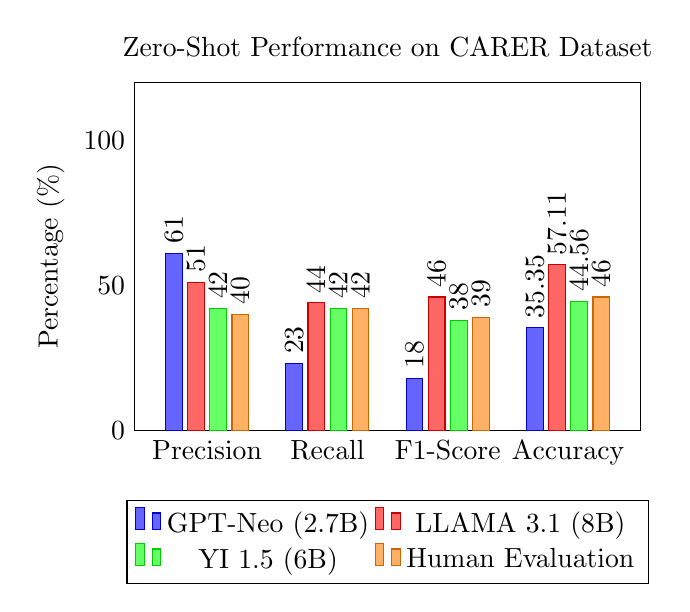
\begin{tikzpicture}
    \begin{axis}[
        legend style={at={(0.5,-0.2)}, anchor=north, legend columns=2},
        symbolic x coords={Precision,Recall,F1-Score,Accuracy},
        major tick length=0cm,
        xtick=data,
        ymin=0,
        ymax=100.0,
        enlarge x limits=0.2,
        enlarge y limits={upper,value=0.2},
        nodes near coords,
        ybar,
        every node near coord/.append style={rotate=90, anchor=west},
        bar width = 6pt,
        ylabel={Percentage (\%)},
        title={Zero-Shot Performance on CARER Dataset},
        width=8cm,
        height=6cm,
        error bars/y dir=both,
        error bars/y explicit,
        error bars/error bar style={line width=1pt},
    ]
        \addplot[fill=blue!60, draw=blue!80!black]
            coordinates {
                (Precision,61) (Recall,23) (F1-Score,18) (Accuracy,35.35)
            };
        \addplot[fill=red!60, draw=red!80!black]
            coordinates {
                (Precision,51) (Recall,44) (F1-Score,46) (Accuracy,57.105)
            };
        \addplot[fill=green!60, draw=green!80!black]
            coordinates {
                (Precision,42) (Recall,42) (F1-Score,38) (Accuracy,44.558)
            };
        \addplot[fill=orange!60, draw=orange!80!black]
            coordinates {
                (Precision,40) (Recall,42) (F1-Score,39) (Accuracy,46)
            };
        
        \legend{GPT-Neo (2.7B),LLAMA 3.1 (8B),YI 1.5 (6B),Human Evaluation}
    \end{axis}
\end{tikzpicture}



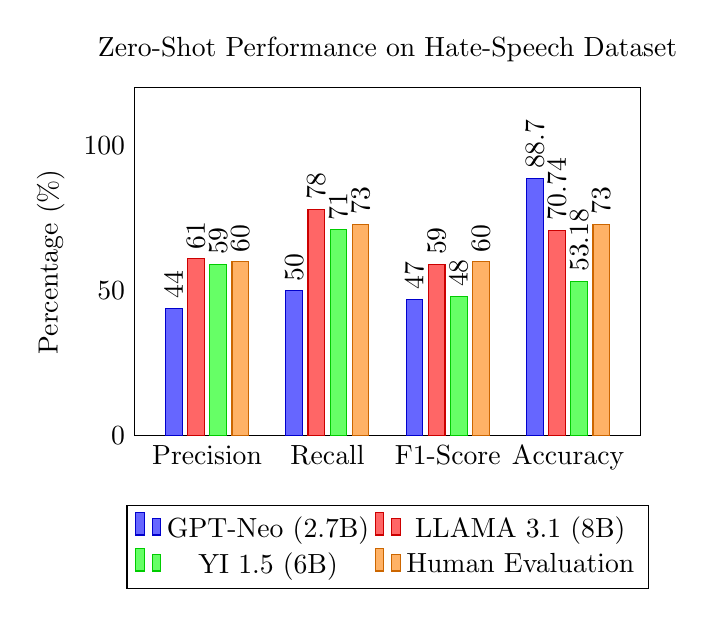
\begin{tikzpicture}
    \begin{groupplot}[
        group style={
            group size=2 by 1,
            horizontal sep=2cm
        },
        width=8cm,
        height=6cm
    ]
        \nextgroupplot[
            legend style={at={(0.5,-0.2)}, anchor=north, legend columns=2},
            symbolic x coords={Precision,Recall,F1-Score,Accuracy},
            major tick length=0cm,
            xtick=data,
            ymin=0.0,
            ymax=100.0,
            enlarge x limits=0.2,
            enlarge y limits={upper,value=0.2},
            nodes near coords={\pgfmathprintnumber\pgfplotspointmeta},
            ybar,
            every node near coord/.append style={rotate=90, anchor=west},
            bar width = 6pt,
            ylabel={Percentage (\%)},
            title={Zero-Shot Performance on Hate-Speech Dataset}
        ]
        \addplot[fill=blue!60, draw=blue!80!black]
            coordinates {
                (Precision,44)
                (Recall,50)
                (F1-Score,47)
                (Accuracy,88.7)
            };
        \addplot[fill=red!60, draw=red!80!black]
            coordinates {
                (Precision,61)
                (Recall,78)
                (F1-Score,59)
                (Accuracy,70.74)
            };
        \addplot[fill=green!60, draw=green!80!black]
            coordinates {
                (Precision,59)
                (Recall,71)
                (F1-Score,48)
                (Accuracy,53.18)
            };
        \addplot[fill=orange!60, draw=orange!80!black]
            coordinates {
                (Precision,60)
                (Recall,73)
                (F1-Score,60)
                (Accuracy,73)
            };
        
        \legend{GPT-Neo (2.7B),LLAMA 3.1 (8B),YI 1.5 (6B),Human Evaluation}
    \end{groupplot}
\end{tikzpicture}


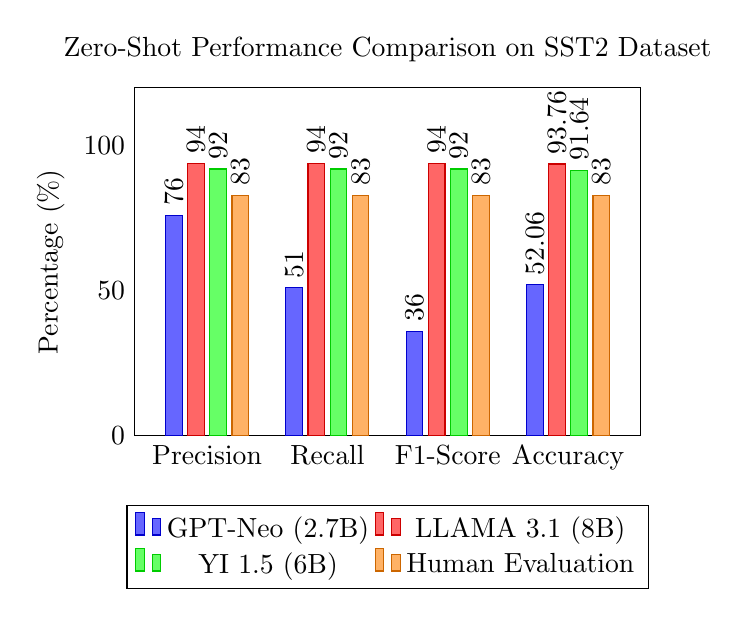
\begin{tikzpicture}
    \begin{groupplot}[
        group style={
            group size=2 by 1,
            horizontal sep=2cm
        },
        width=8cm,
        height=6cm
    ]
        \nextgroupplot[
            legend style={at={(0.5,-0.2)}, anchor=north, legend columns=2},
            symbolic x coords={Precision,Recall,F1-Score,Accuracy},
            major tick length=0cm,
            xtick=data,
            ymin=0.0,
            ymax=100.0,
            enlarge x limits=0.2,
            enlarge y limits={upper,value=0.2},
            nodes near coords={\pgfmathprintnumber\pgfplotspointmeta},
            ybar,
            every node near coord/.append style={rotate=90, anchor=west},
            bar width = 6pt,
            ylabel={Percentage (\%)},
            title={Zero-Shot Performance Comparison on SST2 Dataset}
        ]
        \addplot[fill=blue!60, draw=blue!80!black]
            coordinates {
                (Precision,76)
                (Recall,51)
                (F1-Score,36)
                (Accuracy,52.06)
            };
        \addplot[fill=red!60, draw=red!80!black]
            coordinates {
                (Precision,94)
                (Recall,94)
                (F1-Score,94)
                (Accuracy,93.76)
            };
        \addplot[fill=green!60, draw=green!80!black]
            coordinates {
                (Precision,92)
                (Recall,92)
                (F1-Score,92)
                (Accuracy,91.64)
            };
        \addplot[fill=orange!60, draw=orange!80!black]
            coordinates {
                (Precision,83)
                (Recall,83)
                (F1-Score,83)
                (Accuracy,83)
            };
        
        \legend{GPT-Neo (2.7B),LLAMA 3.1 (8B),YI 1.5 (6B),Human Evaluation}
    \end{groupplot}
\end{tikzpicture}


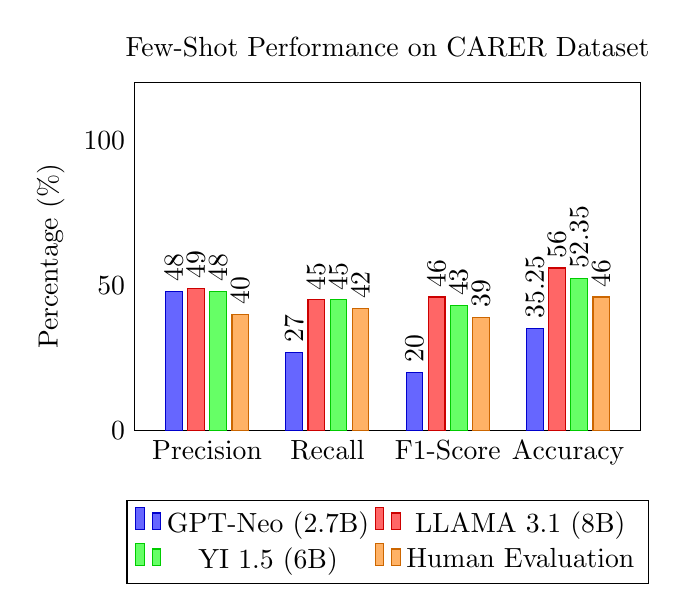
\begin{tikzpicture}
    \begin{axis}[
        legend style={at={(0.5,-0.2)}, anchor=north, legend columns=2},
        symbolic x coords={Precision,Recall,F1-Score,Accuracy},
        major tick length=0cm,
        xtick=data,
        ymin=0,
        ymax=100.0,
        enlarge x limits=0.2,
        enlarge y limits={upper,value=0.2},
        nodes near coords,
        ybar,
        every node near coord/.append style={rotate=90, anchor=west},
        bar width = 6pt,
        ylabel={Percentage (\%)},
        title={Few-Shot Performance on CARER Dataset},
        width=8cm,
        height=6cm,
        error bars/y dir=both,
        error bars/y explicit,
        error bars/error bar style={line width=1pt},
    ]
        \addplot[fill=blue!60, draw=blue!80!black]
            coordinates {
                (Precision,48) (Recall,27) (F1-Score,20) (Accuracy,35.25)
            };
        \addplot[fill=red!60, draw=red!80!black]
            coordinates {
                (Precision,49) (Recall,45) (F1-Score,46) (Accuracy,56.00)
            };
        \addplot[fill=green!60, draw=green!80!black]
            coordinates {
                (Precision,48) (Recall,45) (F1-Score,43) (Accuracy,52.35)
            };
        \addplot[fill=orange!60, draw=orange!80!black]
            coordinates {
                (Precision,40) (Recall,42) (F1-Score,39) (Accuracy,46)
            };
        
        \legend{GPT-Neo (2.7B),LLAMA 3.1 (8B),YI 1.5 (6B),Human Evaluation}
    \end{axis}
\end{tikzpicture}

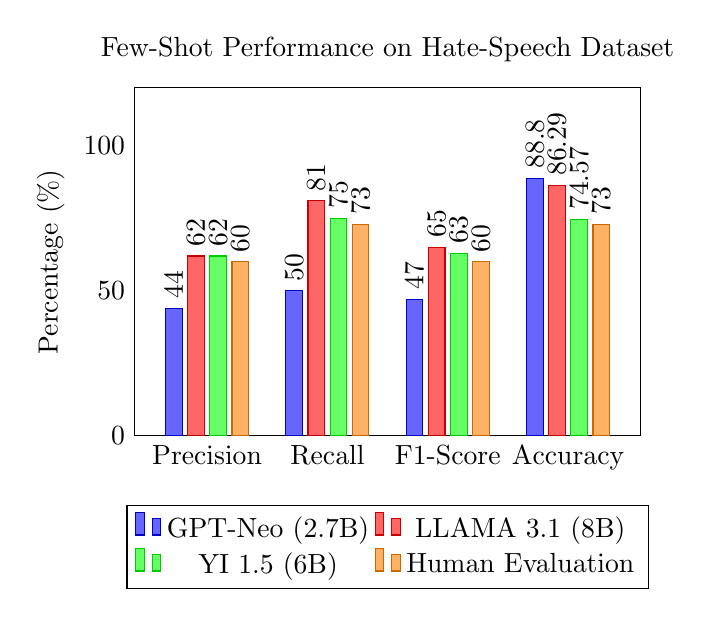
\begin{tikzpicture}
    \begin{axis}[
        legend style={at={(0.5,-0.2)}, anchor=north, legend columns=2},
        symbolic x coords={Precision,Recall,F1-Score,Accuracy},
        major tick length=0cm,
        xtick=data,
        ymin=0,
        ymax=100.0,
        enlarge x limits=0.2,
        enlarge y limits={upper,value=0.2},
        nodes near coords,
        ybar,
        every node near coord/.append style={rotate=90, anchor=west},
        bar width = 6pt,
        ylabel={Percentage (\%)},
        title={Few-Shot Performance on Hate-Speech Dataset},
        width=8cm,
        height=6cm,
        error bars/y dir=both,
        error bars/y explicit,
        error bars/error bar style={line width=1pt},
    ]
        \addplot[fill=blue!60, draw=blue!80!black]
            coordinates {
                (Precision,44) (Recall,50) (F1-Score,47) (Accuracy,88.8)
            };
        \addplot[fill=red!60, draw=red!80!black]
            coordinates {
                (Precision,62) (Recall,81) (F1-Score,65) (Accuracy,86.29)
            };
        \addplot[fill=green!60, draw=green!80!black]
            coordinates {
                (Precision,62) (Recall,75) (F1-Score,63) (Accuracy,74.57)
            };
        \addplot[fill=orange!60, draw=orange!80!black]
            coordinates {
                (Precision,60) (Recall,73) (F1-Score,60) (Accuracy,73)
            };
        
        \legend{GPT-Neo (2.7B),LLAMA 3.1 (8B),YI 1.5 (6B),Human Evaluation}
    \end{axis}
\end{tikzpicture}


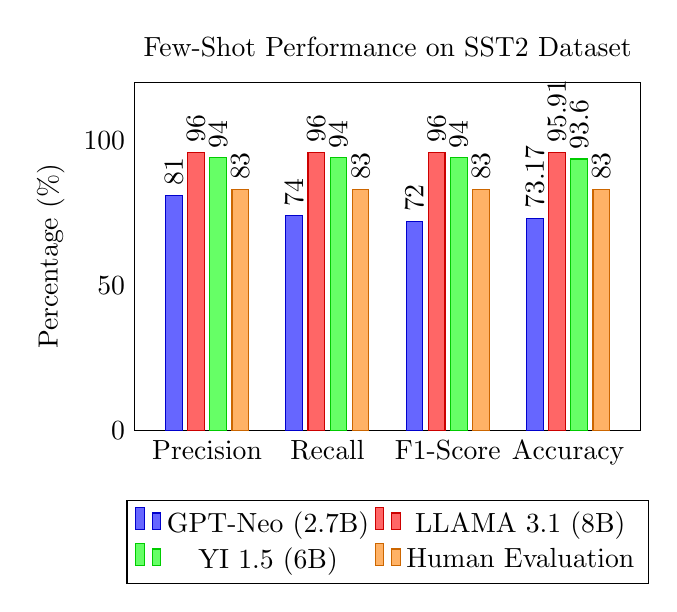
\begin{tikzpicture}
    \begin{axis}[
        legend style={at={(0.5,-0.2)}, anchor=north, legend columns=2},
        symbolic x coords={Precision,Recall,F1-Score,Accuracy},
        major tick length=0cm,
        xtick=data,
        ymin=0,
        ymax=100.0,
        enlarge x limits=0.2,
        enlarge y limits={upper,value=0.2},
        nodes near coords,
        ybar,
        every node near coord/.append style={rotate=90, anchor=west},
        bar width = 6pt,
        ylabel={Percentage (\%)},
        title={Few-Shot Performance on SST2 Dataset},
        width=8cm,
        height=6cm,
        error bars/y dir=both,
        error bars/y explicit,
        error bars/error bar style={line width=1pt},
    ]
        \addplot[fill=blue!60, draw=blue!80!black]
            coordinates {
                (Precision,81) (Recall,74) (F1-Score,72) (Accuracy,73.17)
            };
        \addplot[fill=red!60, draw=red!80!black]
            coordinates {
                (Precision,96) (Recall,96) (F1-Score,96) (Accuracy,95.91)
            };
        \addplot[fill=green!60, draw=green!80!black]
            coordinates {
                (Precision,94) (Recall,94) (F1-Score,94) (Accuracy,93.60)
            };
        \addplot[fill=orange!60, draw=orange!80!black]
            coordinates {
                (Precision,83) (Recall,83) (F1-Score,83) (Accuracy,83)
            };
        
        \legend{GPT-Neo (2.7B),LLAMA 3.1 (8B),YI 1.5 (6B),Human Evaluation}
    \end{axis}
\end{tikzpicture}


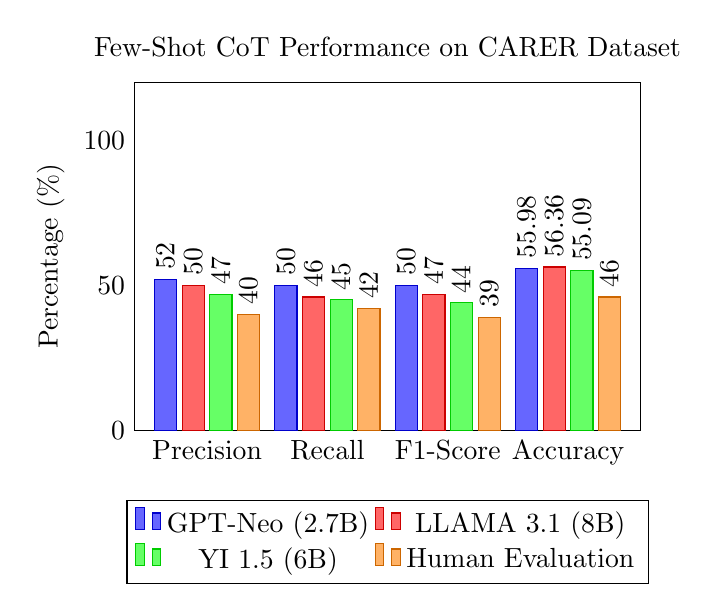
\begin{tikzpicture}
    \begin{axis}[
        legend style={at={(0.5,-0.2)}, anchor=north, legend columns=2},
        symbolic x coords={Precision,Recall,F1-Score,Accuracy},
        major tick length=0cm,
        xtick=data,
        ymin=0,
        ymax=100.0,
        enlarge x limits=0.2,
        enlarge y limits={upper,value=0.2},
        nodes near coords,
        ybar,
        every node near coord/.append style={rotate=90, anchor=west},
        bar width = 8pt,
        ylabel={Percentage (\%)},
        title={Few-Shot CoT Performance on CARER Dataset},
        width=8cm,
        height=6cm,
        error bars/y dir=both,
        error bars/y explicit,
        error bars/error bar style={line width=1pt},
    ]
        \addplot[fill=blue!60, draw=blue!80!black]
            coordinates {
                (Precision,52) (Recall,50) (F1-Score,50) (Accuracy,55.98)
            };
        \addplot[fill=red!60, draw=red!80!black]
            coordinates {
                (Precision,50) (Recall,46) (F1-Score,47) (Accuracy,56.36)
            };
        \addplot[fill=green!60, draw=green!80!black]
            coordinates {
                (Precision,47) (Recall,45) (F1-Score,44) (Accuracy,55.09)
            };
        \addplot[fill=orange!60, draw=orange!80!black]
            coordinates {
                (Precision,40) (Recall,42) (F1-Score,39) (Accuracy,46)
            };
        
        \legend{GPT-Neo (2.7B),LLAMA 3.1 (8B),YI 1.5 (6B),Human Evaluation}
    \end{axis}
\end{tikzpicture}

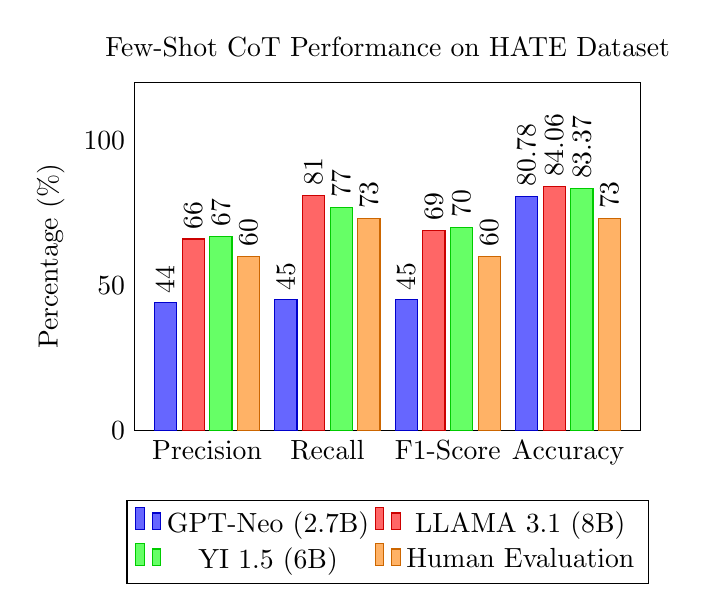
\begin{tikzpicture}
    \begin{axis}[
        legend style={at={(0.5,-0.2)}, anchor=north, legend columns=2},
        symbolic x coords={Precision,Recall,F1-Score,Accuracy},
        major tick length=0cm,
        xtick=data,
        ymin=0,
        ymax=100.0,
        enlarge x limits=0.2,
        enlarge y limits={upper,value=0.2},
        nodes near coords,
        ybar,
        every node near coord/.append style={rotate=90, anchor=west},
        bar width = 8pt,
        ylabel={Percentage (\%)},
        title={Few-Shot CoT Performance on HATE Dataset},
        width=8cm,
        height=6cm,
        error bars/y dir=both,
        error bars/y explicit,
        error bars/error bar style={line width=1pt},
    ]
        \addplot[fill=blue!60, draw=blue!80!black]
            coordinates {
                (Precision,44) (Recall,45) (F1-Score,45) (Accuracy,80.78)
            };
        \addplot[fill=red!60, draw=red!80!black]
            coordinates {
                (Precision,66) (Recall,81) (F1-Score,69) (Accuracy,84.06)
            };
        \addplot[fill=green!60, draw=green!80!black]
            coordinates {
                (Precision,67) (Recall,77) (F1-Score,70) (Accuracy,83.37)
            };
        \addplot[fill=orange!60, draw=orange!80!black]
            coordinates {
                (Precision,60) (Recall,73) (F1-Score,60) (Accuracy,73)
            };
        
        \legend{GPT-Neo (2.7B),LLAMA 3.1 (8B),YI 1.5 (6B),Human Evaluation}
    \end{axis}
\end{tikzpicture}

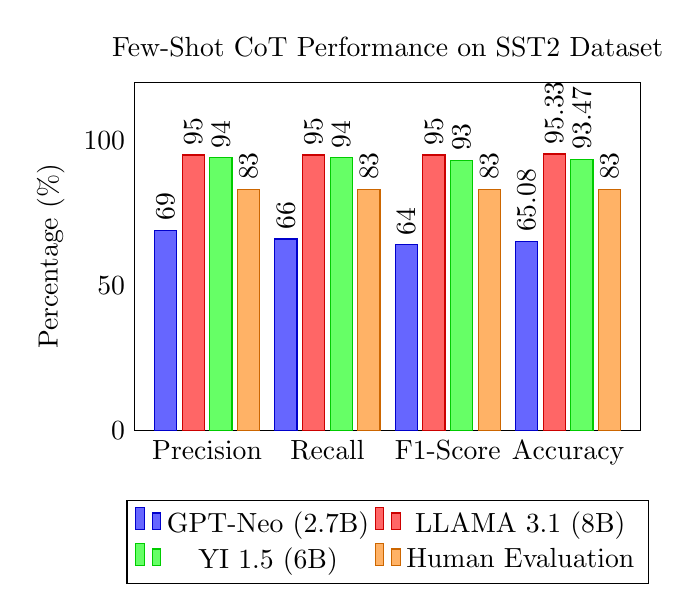
\begin{tikzpicture}
    \begin{axis}[
        legend style={at={(0.5,-0.2)}, anchor=north, legend columns=2},
        symbolic x coords={Precision,Recall,F1-Score,Accuracy},
        major tick length=0cm,
        xtick=data,
        ymin=0,
        ymax=100.0,
        enlarge x limits=0.2,
        enlarge y limits={upper,value=0.2},
        nodes near coords,
        ybar,
        every node near coord/.append style={rotate=90, anchor=west},
        bar width = 8pt,
        ylabel={Percentage (\%)},
        title={Few-Shot CoT Performance on SST2 Dataset},
        width=8cm,
        height=6cm,
        error bars/y dir=both,
        error bars/y explicit,
        error bars/error bar style={line width=1pt},
    ]
        \addplot[fill=blue!60, draw=blue!80!black]
            coordinates {
                (Precision,69) (Recall,66) (F1-Score,64) (Accuracy,65.08)
            };
        \addplot[fill=red!60, draw=red!80!black]
            coordinates {
                (Precision,95) (Recall,95) (F1-Score,95) (Accuracy,95.33)
            };
        \addplot[fill=green!60, draw=green!80!black]
            coordinates {
                (Precision,94) (Recall,94) (F1-Score,93) (Accuracy,93.47)
            };
        \addplot[fill=orange!60, draw=orange!80!black]
            coordinates {
                (Precision,83) (Recall,83) (F1-Score,83) (Accuracy,83)
            };
        
        \legend{GPT-Neo (2.7B),LLAMA 3.1 (8B),YI 1.5 (6B),Human Evaluation}
    \end{axis}
\end{tikzpicture}

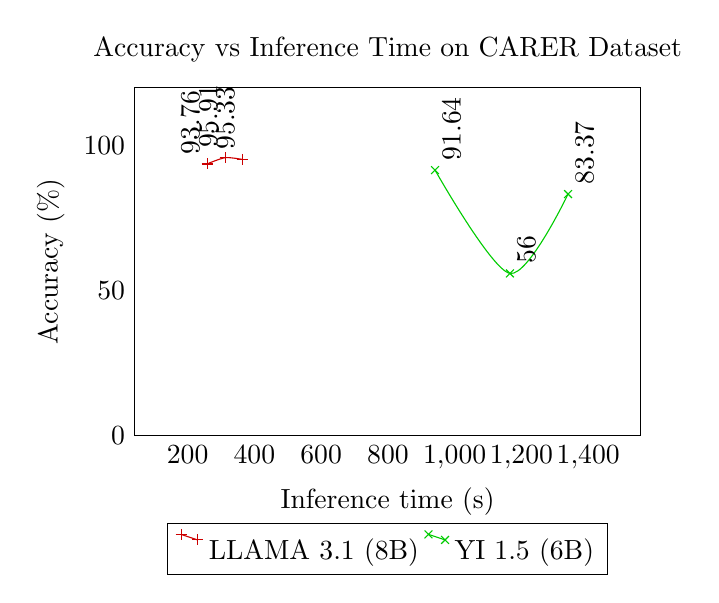
\begin{tikzpicture}
    \begin{axis}[
        legend style={at={(0.5,-0.25)}, anchor=north, legend columns=2},
        major tick length=0cm,
        % xtick=data,
        ymin=0,
        ymax=100.0,
        enlarge x limits=0.2,
        enlarge y limits={upper,value=0.2},
        nodes near coords,
        ybar,
        every node near coord/.append style={rotate=90, anchor=west},
        xlabel={Inference time (s)},
        ylabel={Accuracy (\%)},
        title={Accuracy vs Inference Time on CARER Dataset},
        width=8cm,
        height=6cm,
    ]
    
    \addplot[smooth,mark=+,draw=red!80!black]
        plot coordinates {
            (258.14, 93.76)
            (312.43, 95.91)
            (363.24, 95.33)
        };
        \addlegendentry{LLAMA 3.1 (8B)}
        
    \addplot[smooth,mark=x,draw=green!80!black]
        plot coordinates {
            (941.18, 91.64)
            (1165.56, 56.00)
            (1339.65, 83.37)
        };
        \addlegendentry{YI 1.5 (6B)}
        
    \end{axis}
\end{tikzpicture}

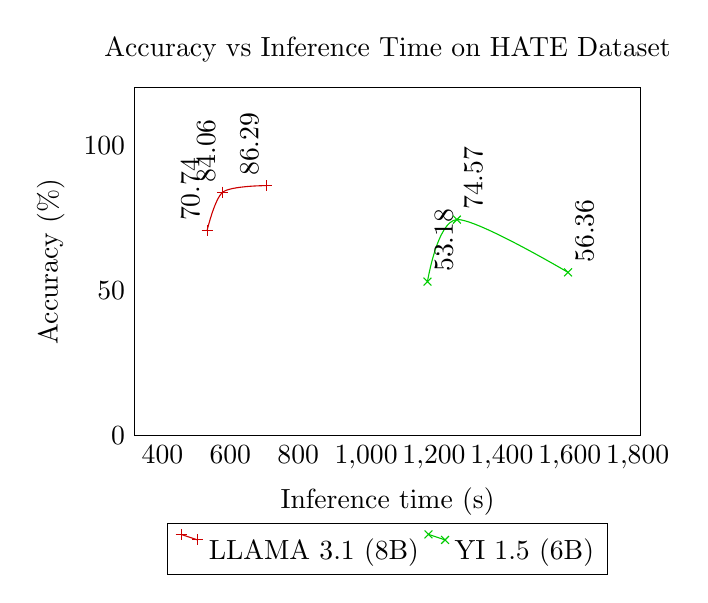
\begin{tikzpicture}
    \begin{axis}[
        legend style={at={(0.5,-0.25)}, anchor=north, legend columns=2},
        major tick length=0cm,
        % xtick=data,
        ymin=0,
        ymax=100.0,
        enlarge x limits=0.2,
        enlarge y limits={upper,value=0.2},
        nodes near coords,
        ybar,
        every node near coord/.append style={rotate=90, anchor=west},
        xlabel={Inference time (s)},
        ylabel={Accuracy (\%)},
        title={Accuracy vs Inference Time on HATE Dataset},
        width=8cm,
        height=6cm,
    ]
    
    \addplot[smooth,mark=+,draw=red!80!black]
        plot coordinates {
            (531.48,70.74)
            (578.11,84.06)
            (705.41,86.29)
        };
        \addlegendentry{LLAMA 3.1 (8B)}
        
    \addplot[smooth,mark=x,draw=green!80!black]
        plot coordinates {
            (1180.74, 53.18)
            (1267.44, 74.57)
            (1594.84, 56.36)
        };
        \addlegendentry{YI 1.5 (6B)}
        
    \end{axis}
\end{tikzpicture}

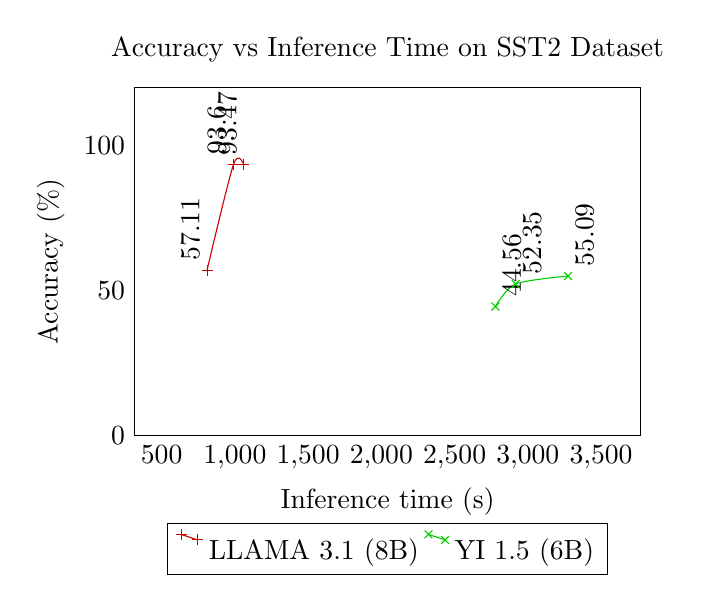
\begin{tikzpicture}
    \begin{axis}[
        legend style={at={(0.5,-0.25)}, anchor=north, legend columns=2},
        major tick length=0cm,
        % xtick=data,
        ymin=0,
        ymax=100.0,
        enlarge x limits=0.2,
        enlarge y limits={upper,value=0.2},
        nodes near coords,
        ybar,
        every node near coord/.append style={rotate=90, anchor=west},
        xlabel={Inference time (s)},
        ylabel={Accuracy (\%)},
        title={Accuracy vs Inference Time on SST2 Dataset},
        width=8cm,
        height=6cm,
    ]
    
    \addplot[smooth,mark=+,draw=red!80!black]
        plot coordinates {
            (810.19, 57.11)
            (990.96, 93.60)
            (1061.99, 93.47)
        };
        \addlegendentry{LLAMA 3.1 (8B)}
        
    \addplot[smooth,mark=x,draw=green!80!black]
        plot coordinates {
            (2778.79, 44.56)
            (2916.41, 52.35)
            (3274.68, 55.09)
        };
        \addlegendentry{YI 1.5 (6B)}
        
    \end{axis}
\end{tikzpicture}

\onecolumn

\newpage

\begin{sidewaystable}[ht]
\centering
\caption{Model Performance Across Prompting Techniques on the \textbf{CARER} Dataset}
\vspace{10pt}
\label{tab:model_performance_carer}
\begin{NiceTabular}{cl*{6}{c}}[corners,hvlines,cell-space-limits=6pt]
    &   \Block{2-1}{}
        & \Block{1-*}{\textbf{Metrics}} \\
    & \textbf{Model}  
        & Accuracy & Precision & Recall & F1-Score & Support & Filtered \\

\Block{2-1}<\rotate>{Baseline}
	 & \textsc{BART (139M)} & 92.83 & 0.93 & 0.85 & 0.88 & 2000 & 0 \\
	 & \textsc{T5 (223M)} & 93.0 & 0.9 & 0.86 & 0.88 & 2000 & 0 \\

\Block{3-1}<\rotate>{Zero-Shot}
	 & \textsc{GPT-Neo (2.7B)} & 35.35 (\textcolor{Red}{-57.48}, \textcolor{Red}{-57.65}) & 0.61 (\textcolor{Red}{-0.32}, \textcolor{Red}{-0.29}) & 0.23 (\textcolor{Red}{-0.62}, \textcolor{Red}{-0.63}) & 0.18 (\textcolor{Red}{-0.7}, \textcolor{Red}{-0.7}) & 2000 & N/A \\
	 & \textsc{LLAMA 3.1 (8B)} & 57.10 (\textcolor{Red}{-35.72}, \textcolor{Red}{-35.9}) & 0.51 (\textcolor{Red}{-0.42}, \textcolor{Red}{-0.39}) & 0.44 (\textcolor{Red}{-0.41}, \textcolor{Red}{-0.42}) & 0.46 (\textcolor{Red}{-0.42}, \textcolor{Red}{-0.42}) & 1886 & 114 \\
	 & \textsc{YI 1.5 (6B)} & 44.56 (\textcolor{Red}{-48.27}, \textcolor{Red}{-48.44}) & 0.42 (\textcolor{Red}{-0.51}, \textcolor{Red}{-0.48}) & 0.42 (\textcolor{Red}{-0.43}, \textcolor{Red}{-0.44}) & 0.38 (\textcolor{Red}{-0.5}, \textcolor{Red}{-0.5}) & 1957 & 43 \\

\Block{3-1}<\rotate>{Few-Shot}
	 & \textsc{GPT-Neo (2.7B)} & 35.25 (\textcolor{Red}{-57.58}, \textcolor{Red}{-57.75}) & 0.48 (\textcolor{Red}{-0.45}, \textcolor{Red}{-0.42}) & 0.27 (\textcolor{Red}{-0.58}, \textcolor{Red}{-0.59}) & 0.20 (\textcolor{Red}{-0.68}, \textcolor{Red}{-0.68}) & 2000 & N/A \\
	 & \textsc{LLAMA 3.1 (8B)} & 56.00 (\textcolor{Red}{-36.83}, \textcolor{Red}{-37.0}) & 0.49 (\textcolor{Red}{-0.44}, \textcolor{Red}{-0.41}) & 0.45 (\textcolor{Red}{-0.4}, \textcolor{Red}{-0.41}) & 0.46 (\textcolor{Red}{-0.42}, \textcolor{Red}{-0.42}) & 1916 & 84 \\
	 & \textsc{YI 1.5 (6B)} & 52.35 (\textcolor{Red}{-40.48}, \textcolor{Red}{-40.65}) & 0.48 (\textcolor{Red}{-0.45}, \textcolor{Red}{-0.42}) & 0.45 (\textcolor{Red}{-0.4}, \textcolor{Red}{-0.41}) & 0.43 (\textcolor{Red}{-0.45}, \textcolor{Red}{-0.45}) & 1912 & 88 \\

\Block{3-1}<\rotate>{Few-Shot CoT}
	 & \textsc{GPT-Neo (2.7B)} & 55.98 (\textcolor{Red}{-36.85}, \textcolor{Red}{-37.02}) & 0.52 (\textcolor{Red}{-0.41}, \textcolor{Red}{-0.38}) & 0.50 (\textcolor{Red}{-0.35}, \textcolor{Red}{-0.36}) & 0.50 (\textcolor{Red}{-0.38}, \textcolor{Red}{-0.38}) & 786 & 1214 \\
	 & \textsc{LLAMA 3.1 (8B)} & 56.36 (\textcolor{Red}{-36.47}, \textcolor{Red}{-36.64}) & 0.50 (\textcolor{Red}{-0.43}, \textcolor{Red}{-0.4}) & 0.46 (\textcolor{Red}{-0.39}, \textcolor{Red}{-0.4}) & 0.47 (\textcolor{Red}{-0.41}, \textcolor{Red}{-0.41}) & 1909 & 91 \\
	 & \textsc{YI 1.5 (6B)} & 55.09 (\textcolor{Red}{-37.74}, \textcolor{Red}{-37.91}) & 0.47 (\textcolor{Red}{-0.46}, \textcolor{Red}{-0.43}) & 0.45 (\textcolor{Red}{-0.4}, \textcolor{Red}{-0.41}) & 0.44 (\textcolor{Red}{-0.44}, \textcolor{Red}{-0.44}) & 1886 & 114 \\

	 & \textsc{Human Evaluation} & 46.00 (\textcolor{Red}{-46.83}, \textcolor{Red}{-47.0}) & 0.40 (\textcolor{Red}{-0.53}, \textcolor{Red}{-0.5}) & 0.42 (\textcolor{Red}{-0.43}, \textcolor{Red}{-0.44}) & 0.39 (\textcolor{Red}{-0.49}, \textcolor{Red}{-0.49}) & 400 & 0 \\

\end{NiceTabular}
\end{sidewaystable}

\begin{sidewaystable}[ht]
\centering
\caption{Model Performance Across Prompting Techniques on the \textbf{Hate Speech} Dataset}
\vspace{10pt}
\label{tab:model_performance_hate_speech}
\begin{NiceTabular}{cl*{6}{c}}[corners,hvlines,cell-space-limits=6pt]
    &   \Block{2-1}{}
        & \Block{1-*}{\textbf{Metrics}} \\
    & \textbf{Model}  
        & Accuracy & Precision & Recall & F1-Score & Support & Filtered \\

\Block{2-1}<\rotate>{Baseline}
	 & \textsc{BART (139M)} & 90.94 & 0.79 & 0.74 & 0.76 & 1071 & 0 \\
	 & \textsc{T5 (223M)} & 92.2 & 0.81 & 0.76 & 0.79 & 1071 & 0 \\

\Block{3-1}<\rotate>{Zero-Shot}
	 & \textsc{GPT-Neo (2.7B)} & 88.70 (\textcolor{Red}{-2.24}, \textcolor{Red}{-3.5}) & 0.44 (\textcolor{Red}{-0.35}, \textcolor{Red}{-0.37}) & 0.50 (\textcolor{Red}{-0.24}, \textcolor{Red}{-0.26}) & 0.47 (\textcolor{Red}{-0.29}, \textcolor{Red}{-0.32}) & 1071 & N/A \\
	 & \textsc{LLAMA 3.1 (8B)} & 70.74 (\textcolor{Red}{-20.2}, \textcolor{Red}{-21.46}) & 0.61 (\textcolor{Red}{-0.18}, \textcolor{Red}{-0.2}) & 0.78 (\textcolor{Green}{0.04}, \textcolor{Green}{0.02}) & 0.59 (\textcolor{Red}{-0.17}, \textcolor{Red}{-0.2}) & 752 & 319 \\
	 & \textsc{YI 1.5 (6B)} & 53.18 (\textcolor{Red}{-37.76}, \textcolor{Red}{-39.02}) & 0.59 (\textcolor{Red}{-0.2}, \textcolor{Red}{-0.22}) & 0.71 (\textcolor{Red}{-0.03}, \textcolor{Red}{-0.05}) & 0.48 (\textcolor{Red}{-0.28}, \textcolor{Red}{-0.31}) & 1006 & 65 \\

\Block{3-1}<\rotate>{Few-Shot}
	 & \textsc{GPT-Neo (2.7B)} & 88.80 (\textcolor{Red}{-2.14}, \textcolor{Red}{-3.4}) & 0.44 (\textcolor{Red}{-0.35}, \textcolor{Red}{-0.37}) & 0.50 (\textcolor{Red}{-0.24}, \textcolor{Red}{-0.26}) & 0.47 (\textcolor{Red}{-0.29}, \textcolor{Red}{-0.32}) & 1071 & N/A \\
	 & \textsc{LLAMA 3.1 (8B)} & 86.29 (\textcolor{Red}{-4.65}, \textcolor{Red}{-5.91}) & 0.62 (\textcolor{Red}{-0.17}, \textcolor{Red}{-0.19}) & 0.81 (\textcolor{Green}{0.07}, \textcolor{Green}{0.05}) & 0.65 (\textcolor{Red}{-0.11}, \textcolor{Red}{-0.14}) & 766 & 305 \\
	 & \textsc{YI 1.5 (6B)} & 74.57 (\textcolor{Red}{-16.37}, \textcolor{Red}{-17.63}) & 0.62 (\textcolor{Red}{-0.17}, \textcolor{Red}{-0.19}) & 0.75 (\textcolor{Green}{0.01}, \textcolor{Red}{-0.01}) & 0.63 (\textcolor{Red}{-0.13}, \textcolor{Red}{-0.16}) & 983 & 88 \\

\Block{3-1}<\rotate>{Few-Shot CoT}
	 & \textsc{GPT-Neo (2.7B)} & 80.78 (\textcolor{Red}{-10.16}, \textcolor{Red}{-11.42}) & 0.44 (\textcolor{Red}{-0.35}, \textcolor{Red}{-0.37}) & 0.45 (\textcolor{Red}{-0.29}, \textcolor{Red}{-0.31}) & 0.45 (\textcolor{Red}{-0.31}, \textcolor{Red}{-0.34}) & 1071 & N/A \\
	 & \textsc{LLAMA 3.1 (8B)} & 84.06 (\textcolor{Red}{-6.88}, \textcolor{Red}{-8.14}) & 0.66 (\textcolor{Red}{-0.13}, \textcolor{Red}{-0.15}) & 0.81 (\textcolor{Green}{0.07}, \textcolor{Green}{0.05}) & 0.69 (\textcolor{Red}{-0.07}, \textcolor{Red}{-0.1}) & 991 & 80 \\
	 & \textsc{YI 1.5 (6B)} & 83.37 (\textcolor{Red}{-7.57}, \textcolor{Red}{-8.83}) & 0.67 (\textcolor{Red}{-0.12}, \textcolor{Red}{-0.14}) & 0.77 (\textcolor{Green}{0.03}, \textcolor{Green}{0.01}) & 0.70 (\textcolor{Red}{-0.06}, \textcolor{Red}{-0.09}) & 1016 & 55 \\

	 & \textsc{Human Evaluation} & 73.00 (\textcolor{Red}{-17.94}, \textcolor{Red}{-19.2}) & 0.60 (\textcolor{Red}{-0.19}, \textcolor{Red}{-0.21}) & 0.73 (\textcolor{Red}{-0.01}, \textcolor{Red}{-0.03}) & 0.60 (\textcolor{Red}{-0.16}, \textcolor{Red}{-0.19}) & 400 & 0 \\

\end{NiceTabular}
\end{sidewaystable}

\begin{sidewaystable}[ht]
\centering
\caption{Model Performance Across Prompting Techniques on the \textbf{SST2} Dataset}
\vspace{10pt}
\label{tab:model_performance_sst2}
\begin{NiceTabular}{cl*{6}{c}}[corners,hvlines,cell-space-limits=6pt]
    &   \Block{2-1}{}
        & \Block{1-*}{\textbf{Metrics}} \\
    & \textbf{Model}  
        & Accuracy & Precision & Recall & F1-Score & Support & Filtered \\

\Block{2-1}<\rotate>{Baseline}
	 & \textsc{BART (139M)} & 93.01 & 0.93 & 0.93 & 0.93 & 872 & 0 \\
	 & \textsc{T5 (223M)} & 93.5 & 0.94 & 0.94 & 0.94 & 872 & 0 \\

\Block{3-1}<\rotate>{Zero-Shot}
	 & \textsc{GPT-Neo (2.7B)} & 52.06 (\textcolor{Red}{-40.95}, \textcolor{Red}{-41.44}) & 0.76 (\textcolor{Red}{-0.17}, \textcolor{Red}{-0.18}) & 0.51 (\textcolor{Red}{-0.42}, \textcolor{Red}{-0.43}) & 0.36 (\textcolor{Red}{-0.57}, \textcolor{Red}{-0.58}) & 872 & N/A \\
	 & \textsc{LLAMA 3.1 (8B)} & 93.76 (\textcolor{Green}{+0.75}, \textcolor{Green}{+0.26}) & 0.94 (\textcolor{Green}{+0.01}, 0.0) & 0.94 (\textcolor{Green}{+0.01}, 0.0) & 0.94 (\textcolor{Green}{+0.01}, 0.0) & 849 & 23 \\
	 & \textsc{YI 1.5 (6B)} & 91.64 (\textcolor{Red}{-1.37}, \textcolor{Red}{-1.86}) & 0.92 (\textcolor{Red}{-0.01}, \textcolor{Red}{-0.02}) & 0.92 (\textcolor{Red}{-0.01}, \textcolor{Red}{-0.02}) & 0.92 (\textcolor{Red}{-0.01}, \textcolor{Red}{-0.02}) & 861 & 11 \\

\Block{3-1}<\rotate>{Few-Shot}
	 & \textsc{GPT-Neo (2.7B)} & 73.17 (\textcolor{Red}{-19.84}, \textcolor{Red}{-20.33}) & 0.81 (\textcolor{Red}{-0.12}, \textcolor{Red}{-0.13}) & 0.74 (\textcolor{Red}{-0.19}, \textcolor{Red}{-0.2}) & 0.72 (\textcolor{Red}{-0.21}, \textcolor{Red}{-0.22}) & 872 & N/A \\
	 & \textsc{LLAMA 3.1 (8B)} & 95.91 (\textcolor{Green}{+2.9}, \textcolor{Green}{+2.41}) & 0.96 (\textcolor{Green}{+0.03}, \textcolor{Green}{+0.02}) & 0.96 (\textcolor{Green}{+0.03}, \textcolor{Green}{+0.02}) & 0.96 (\textcolor{Green}{+0.03}, \textcolor{Green}{+0.02}) & 806 & 66 \\
	 & \textsc{YI 1.5 (6B)} & 93.60 (\textcolor{Green}{+0.59}, \textcolor{Green}{+0.1}) & 0.94 (\textcolor{Green}{+0.01}, 0.0) & 0.94 (\textcolor{Green}{+0.01}, 0.0) & 0.94 (\textcolor{Green}{+0.01}, 0.0) & 828 & 44 \\

\Block{3-1}<\rotate>{Few-Shot CoT}
	 & \textsc{GPT-Neo (2.7B)} & 65.08 (\textcolor{Red}{-27.93}, \textcolor{Red}{-28.42}) & 0.69 (\textcolor{Red}{-0.24}, \textcolor{Red}{-0.25}) & 0.66 (\textcolor{Red}{-0.27}, \textcolor{Red}{-0.28}) & 0.64 (\textcolor{Red}{-0.29}, \textcolor{Red}{-0.3}) & 872 & N/A \\
	 & \textsc{LLAMA 3.1 (8B)} & 95.33 (\textcolor{Green}{+2.32}, \textcolor{Green}{+1.83}) & 0.95 (\textcolor{Green}{+0.02}, \textcolor{Green}{+0.01}) & 0.95 (\textcolor{Green}{+0.02}, \textcolor{Green}{+0.01}) & 0.95 (\textcolor{Green}{+0.02}, \textcolor{Green}{+0.01}) & 814 & 58 \\
	 & \textsc{YI 1.5 (6B)} & 93.47 (\textcolor{Green}{+0.46}, \textcolor{Red}{-0.03}) & 0.94 (\textcolor{Green}{+0.01}, 0.0) & 0.94 (\textcolor{Green}{+0.01}, 0.0) & 0.93 (0.0, \textcolor{Red}{-0.01}) & 827 & 45 \\

	 & \textsc{Human Evaluation} & 83.00 (\textcolor{Red}{-10.01}, \textcolor{Red}{-10.5}) & 0.83 (\textcolor{Red}{-0.1}, \textcolor{Red}{-0.11}) & 0.83 (\textcolor{Red}{-0.1}, \textcolor{Red}{-0.11}) & 0.83 (\textcolor{Red}{-0.1}, \textcolor{Red}{-0.11}) & 400 & 0 \\

\end{NiceTabular}
\end{sidewaystable}

\end{document}
